

% \section{inleiding}%
% Aan de hand van de shortlist die opgemaakt is komt er voor elke geselecteerde managementplatform een proof of concept. Hierbij wordt er gekeken hoe de nodige functionaliteiten werken en toegepast kunnen worden in het systeem.
% Belangrijk om te weten is dat de proof of concept niet de volledige functionaliteit van het managementplatform zal testen. Het doel is om een goed beeld te krijgen van de mogelijkheden en hoe deze kunnen worden toegepast binnen de infrastructuur van Excentis. 
% We verdelen alle managementplatformen in hun eigen subsecties. In deze subsecties worden dan de vooropgestelde testen op uitgevoerd.
% \section{Proxmox VE}%

% Voor deze virtual managementplatform wordt er Proxmox VE 8.4 gebruikt. Dit is de laatste versie van Proxmox VE die op dit moment beschikbaar is.
\section{Proxmox VE}%
\label{sec:ProxomoxVE}
\subsection{cluster opstelling in Proxmox VE}
Voor proxmox VE is er gekozen om te werken met 3 fysieke node's. Zoals beschreven op de officiële documentatiepagina van Proxmox ondersteunt het platform high availability clustering maar moeten er minimaal 3 nodes in de cluster draaien ~\autocite{proxmoxHA}.
Hierbij wordt e rgesproken over minimaal 50\% van de nodes die moeten draaien om de cluster operationeel te houden. Dit is ook de reden waarom er voor 3 nodes is gekozen.
Bij 2 nodes zou er bij een node failure geen quorum zijn en zou de cluster niet meer operationeel zijn. Dit wil zeggen dat er geen 50\% meerderheid is van de cluster die online is. Enkel bij 3 nodes kan er 1 node uitvallen en alsnog meer dan 50 procent online hebben. In zo’n geval wordt er gesproken van een quorum.
In Figuur \ref{fig:cluster-proxmox} wordt de opstelling getoond. Elke node krijgt een unieke naam in de cluster, vaak is dat de hostname zelf.
\begin{figure}[H]
  \centering
  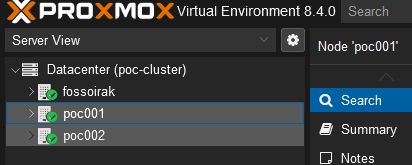
\includegraphics[width=0.85\textwidth]{../poc/cluster-info-prox.png}
  \caption{Clusteropstelling in Proxmox VE}
  \label{fig:cluster-proxmox}
\end{figure}
\subsection{Storage in Proxmox VE}
\label{sec:storage_proxmox}
Proxmox VE ondersteunt verschillende soorten storage. In de proof of concept is er gekozen om te werken met een CEPH storage als distributed storage. Dit is een open-source software-defined storage oplossing die kan worden gebruikt in combinatie met Proxmox VE.
Om deze te configureren moeten er minimaal 3 schijven/partities zijn. Voor deze POC is er besloten om op elke fysieke node een fysieke schijf toe te kennen aan de CEPH storage. Dit zijn 3 willekeurige harde schijven.
Via de GUI kan vanaf elke node worden doorgeklikt naar Ceph. Daar moet worden aangeduid welke schijf gebruikt zal worden voor de Ceph-storage. Dit kan ook via de command line.
Nadat de schijven op elke node zijn toegevoegd, kan via het OSD-menu in de Proxmox-GUI een overzicht worden bekeken, zoals te zien is in Figuur \ref{fig:osd-ceph-proxmox}.
\begin{figure}[H]
  \centering
  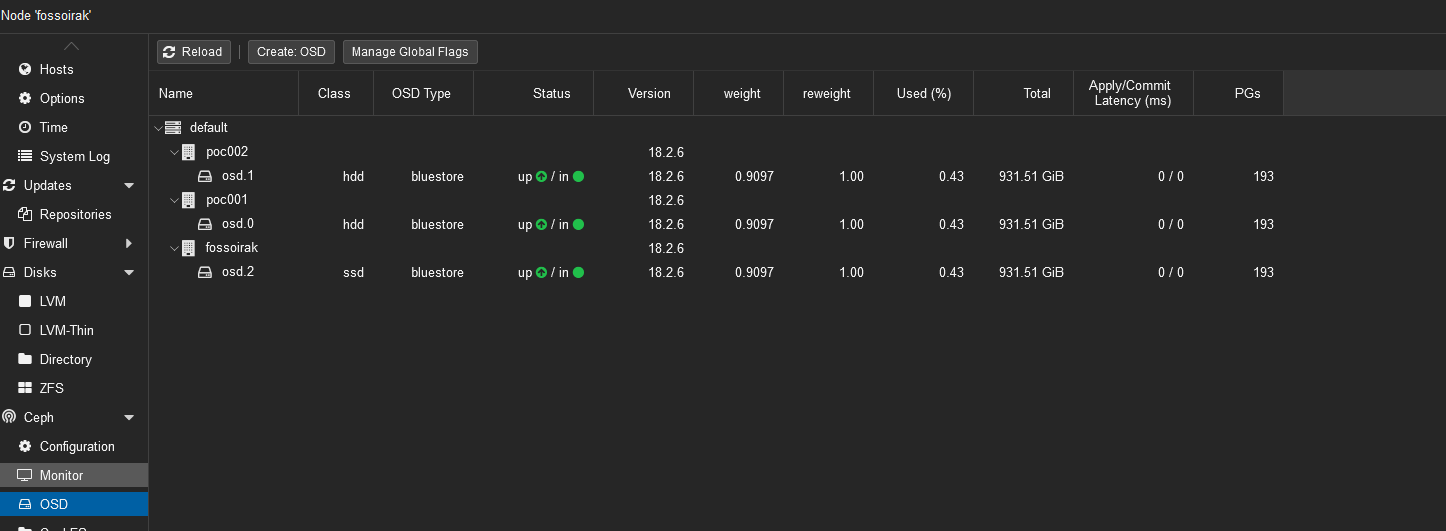
\includegraphics[width=1.0\textwidth, trim=4cm 0cm 4cm 0cm, clip]{../poc/ceph-osd-prox.png}
  \caption{CEPH-schijvenopstelling in Proxmox VE}
  \label{fig:osd-ceph-proxmox}
\end{figure}

Nu kan er een pool aangemaakt worden voor de CEPH storage. Hierin wordt het belangrijste deel van de CEPH configuratie gedaan.
Er wordt aangegeven hoeveel schijven er in de pool moeten zitten. Minimaal zijn dit er hier 3, aangezien er met het HA-systeem wordt gewerkt. Om de HA regels te volgen is het ook essentieel dat er op elke fysieke node een schijf zit voor de pool.
Bij het gebruik van Ceph in Proxmox VE moet het systeem weten hoeveel schijven minimaal beschikbaar moeten zijn om de opslagpool operationeel te houden. Voor deze POC wordt dit ingesteld op 2. Dit is ook de reden waarom er met 3 fysieke nodes is gewerkt. Bij een node failure kan de pool nog steeds gebruikt worden.
De Crush rule in de configuratie is ook belangrijk. Dit is de manier waarop de data verdeeld wordt over de verschillende schijven. Hierin kan ook worden aangegeven dat er een replica van de data op een andere node moet worden gemaakt. Bij een node failure kan de data nog steeds worden benaderd via de andere nodes.
De Figuur \ref{fig:ceph-pool-prox} toont de huidige configuratie van de pool in Proxmox VE.
\begin{figure}[H]
  \centering
  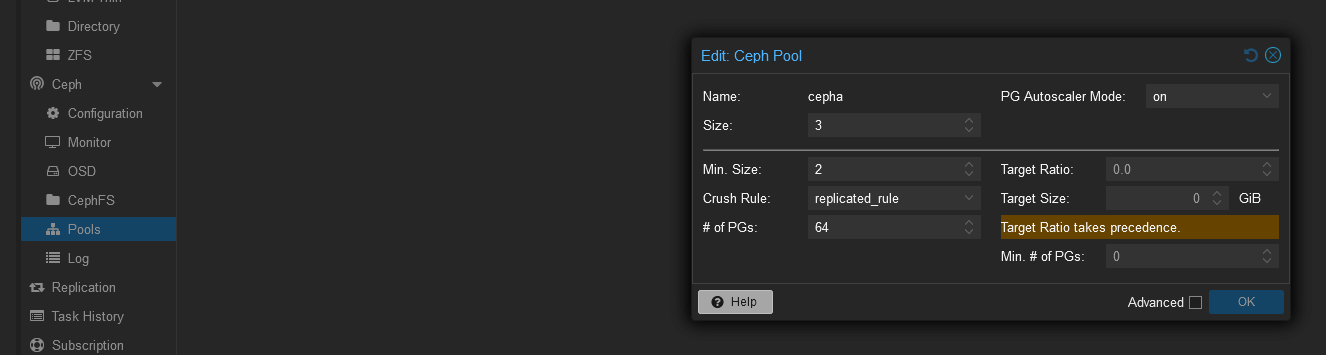
\includegraphics[width=\textwidth, trim=10cm 0cm 0cm 0cm, clip]{../poc/ceph-pool-prox.png}
  \caption{Poolopstelling van CEPH in Proxmox VE}
  \label{fig:ceph-pool-prox}
\end{figure}


Eenmaal aangemaakt kan er een virtuele machine worden aangemakt. Deze virtuele zal Ubuntu 22.04 worden gebruikt als operating system.
De meeste instellingen kunnen helemaal naar keuze worden ingesteld en is voor de rest buiten de scope van deze bachelorproef. De meest relevante instellingen zijn die rond de storage.
Tijdens het configureren van de virtuele machine kan de gewenste schijf worden geselecteerd. Hierbij kan ook de eerder aangemaakte pool worden gekozen.
Merk verder op dat er al een optie is voor SAN iSCSI met TrueNAS~\autocite{truenas} . Deze optie mag tijdelijk genegeerd worden.
Als alles correct is verlopen, kan op alle drie de nodes naar keuze een virtuele machine worden aangemaakt, waarbij overal dezelfde optie beschikbaar is om Ceph als schijfopslag te gebruiken.
Figuur \ref{fig:vm-storage-proxmox} toont de configuratie van de virtuele machine in Proxmox VE.
\begin{figure}[H]
  \centering
  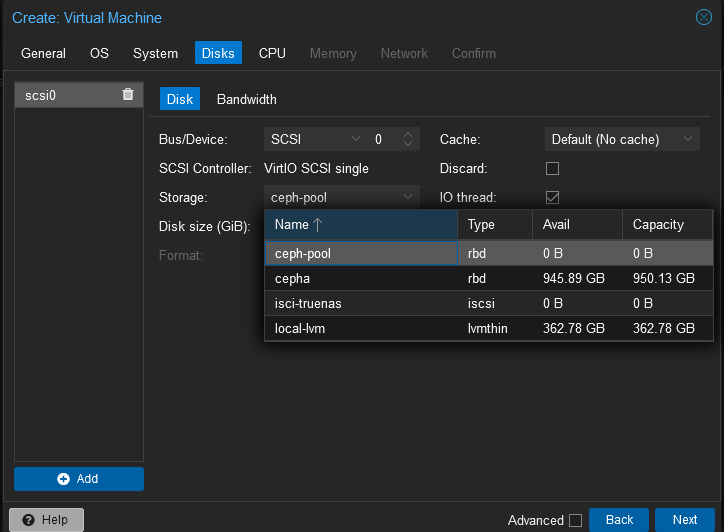
\includegraphics[width=0.85\textwidth, trim=3cm 0cm 3cm 0cm, clip]{../poc/vm-storage-prox.png}
  \caption{VM configuratie met correcte disk in Proxmox VE}
  \label{fig:vm-storage-proxmox}
\end{figure}

De virtuele machine is nu aangemaakt op de node fossoirak.
Ter controle kan er in de GUI onder Datacenter bij de optie CEPH gekeken worden of alle schijven en nodes die de CEPH pool draaien healthy zijn. Zie figur \ref{fig:ceph-healthy-prox}.
Als er geen rode kruisjes staan bij de schijven en nodes is alles perfect geconfigureerd.
\begin{figure}[H]
  \centering
  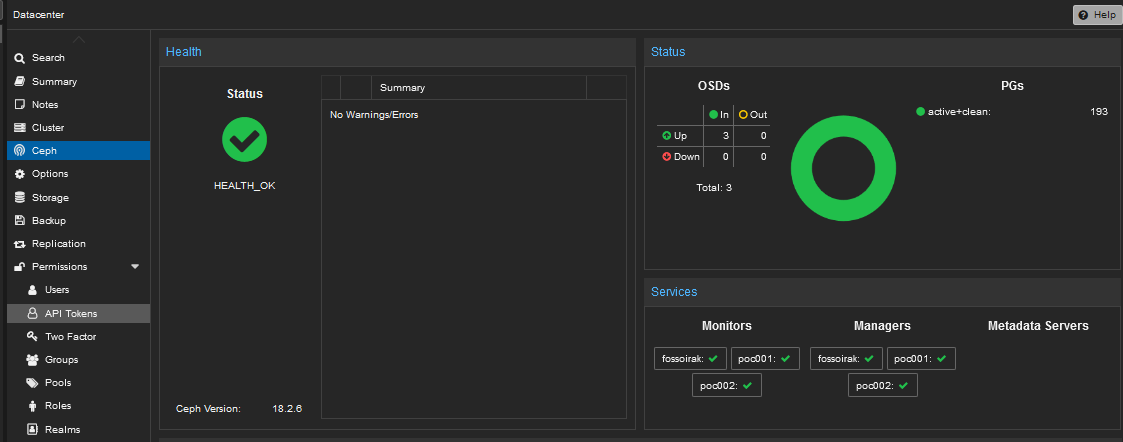
\includegraphics[width=1.1\textwidth]{../poc/ceph-healthy-prox.png}
  \caption{de gezondheid van CEPH  in Proxmox VE}
  \label{fig:ceph-healthy-prox}
\end{figure}

Hierna kan er een HA test uitgevoerd worden. Dit wordt later besproken.
Tijdens het werken met Proxmox VE valt er op dat Proxmox VE automatisch een direct attach storage mount aanmaakt voor te gebruiken. Deze wordt gekoppeld als een directory met als naam local.
Dit toont aan dat Proxmox VE standaard een integratie biedt met DAS. In deze situatie draait het direct op de schijf waar de Proxmox VE zelf op draait zoals te zien is in Figuur \ref{fig:das-prox}.
\begin{figure}[H]
  \centering
  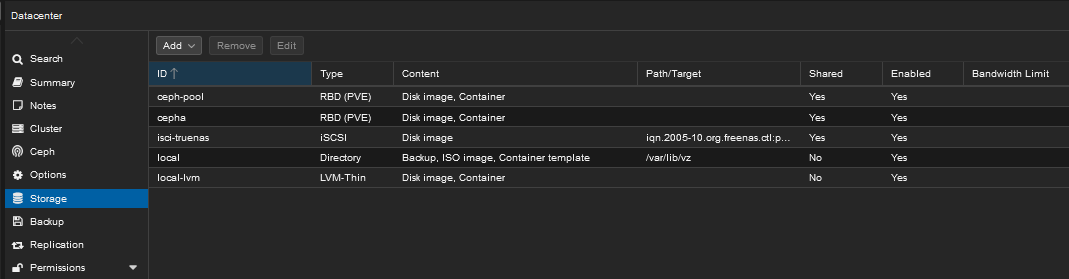
\includegraphics[width=1.1\textwidth]{../poc/das-proxmox.png}
  \caption{direct attach storage in Proxmox VE}
  \label{fig:das-prox}
\end{figure}


Nu is vastgesteld dat CEPH goed werkt, moet er gekeken worden naar de SAN-configuratie met iSCSI.
Er is een bestaande TrueNAS ~\autocite{truenas} server die al draait in de omgeving. Hierop draait een block storage waar iSCI is geconfigureerd.
Onder de tab storage bij Datacenter kan er zeer eenvoudig een iSCSI target worden aangemaakt bij Add, zie Figuur \ref{fig:iscsi-SAN}.
Via de opties in het menu moet er een correct ID als naam worden gegeven en via portal het correct IP adres van de TrueNAS service.
Omdat er gewerkt wordt met een SAN-principe, staat bij de optie node in de configuratie standaard all nodes geselecteerd. Dit is ook de bedoeling, aangezien er met een HA-cluster wordt gewerkt.
De configuratie van iSCI op TrueNAS is buiten de scope van deze bachelorproef.
\begin{figure}[H]
  \centering
  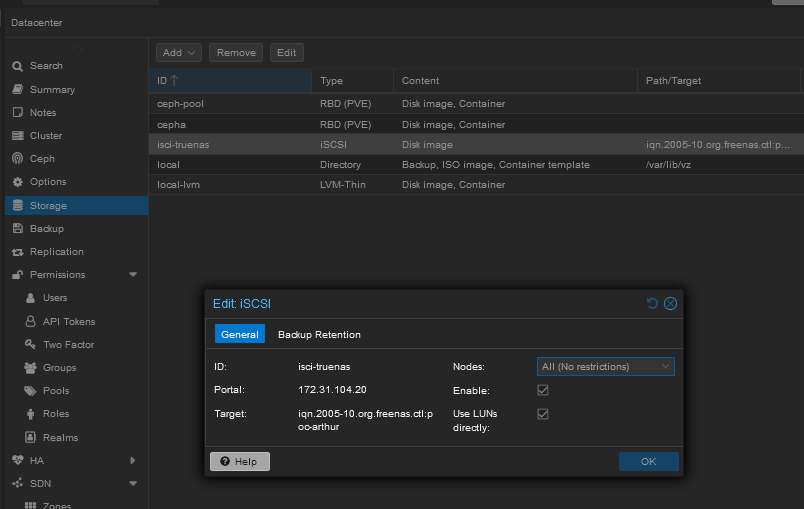
\includegraphics[width=1.0\textwidth]{../poc/iscsi-prox.png}
  \caption{storage area network met ISCI in Proxmox VE}
  \label{fig:iscsi-SAN}
\end{figure}
Nu zal er een extra  optie bijgekomen zijn in de GUI onder de tab storage bij datacenter, zie fiuur~\ref{fig:vm-lijst}  Hier in het voorbeeld wordt het al naam iSCI-TrueNAS gegeven.
Er wordt nu een tweede virtuele machine aangemaakt met dezelfde configuratie als de eerste virtuele machine, maar met een andere schijf. Er wordt nu gekozen voor de isci-truenas disk.
\begin{figure}[H]
  \centering
  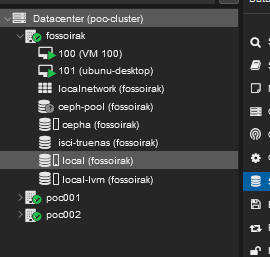
\includegraphics[width=0.85\textwidth]{../poc/vm-lijst-prox.png}
  \caption{Lijst van de 2 virtuele machines in Proxmox VE}
  \label{fig:vm-lijst}
\end{figure}
Aangezien een SAN princiepe via een vebrinding werkt op het netwerk is de storage de zwakste schakel in een high availability cluster. Deze verbinding kan verbroken worden door netwerk problemen. Hierna kan er data corruptie onstaan in het slechtste geval.

\subsection{High Availability in Proxmox VE}
\label{sec:ha-proxmox}
Eenmaal de storage in orde is voor de virtuele machines kan er een HA configuratie worden aangemaakt. 
Onder datacenter HA kan een groep worden aangemaakt. Hierin worden alle drie de fysieke nodes opgenomen die deel uitmaken van de cluster. Vervolgens wordt aan de groep een logische naam toegekend, in dit geval ha-pool zoals in Figuur \ref{fig:ha-group}.
\begin{figure}[H]
  \centering
  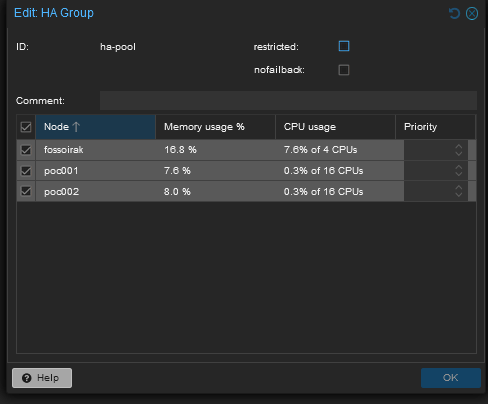
\includegraphics[width=0.85\textwidth]{../poc/ha-group.png}
  \caption{high Availability group in Proxmox VE}
  \label{fig:ha-group}
\end{figure}
De twee virtuele machines worden nu toegevoegd aan de HA-groep. Dit gebeurt via de HA-sectie in Datacenter.
Bij Max Restart en Max Relocate wordt ingesteld hoe vaak een virtuele machine opnieuw mag worden opgestart of verplaatst naar een andere node. In dit geval moet dit groter zijn dan 0 zoals bij Figuur \ref{fig:ha-vm}.
\begin{figure}[H]
  \centering
  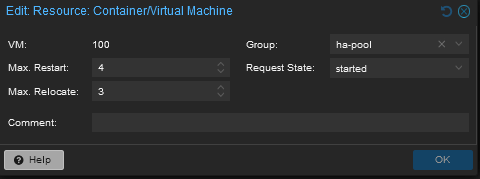
\includegraphics[width=0.85\textwidth]{../poc/vm-ha.png}
  \caption{High Availability vm toevoegen in Proxmox VE}
  \label{fig:ha-vm}
\end{figure}
% Ik heb dit verplaatst naar poc


\section{Xen Orchestra}%
\subsection{Clusteropstelling in Xen Orchestra}
De clusteromgeving van Xen Orchestra met XCP-ng zal weer zoals bij~\ref{sec:ProxomoxVE} bestaan uit 3 fysieke nodes. Elk zal geïnstalleerd worden met XCP-ng 8.3.0.  
De basis wordt opgesteld volgens de documentatie van \textcite{dick2023xcpng}, waarbij Xen Orchestra samen met de drie fysieke nodes wordt geïnstalleerd.  
Figuur \ref{fig:nodes-list} toont de lijst van de nodes die in Xen Orchestra worden beheerd.  
We voegen de nodes ook nog toe aan de pool die is aangemaakt bij het toevoegen van de eerste node. De naam van de pool kan ook nog aangepast worden. In dit geval is de naam van de pool *pool-poc*.

\begin{figure}[H]
  \centering
  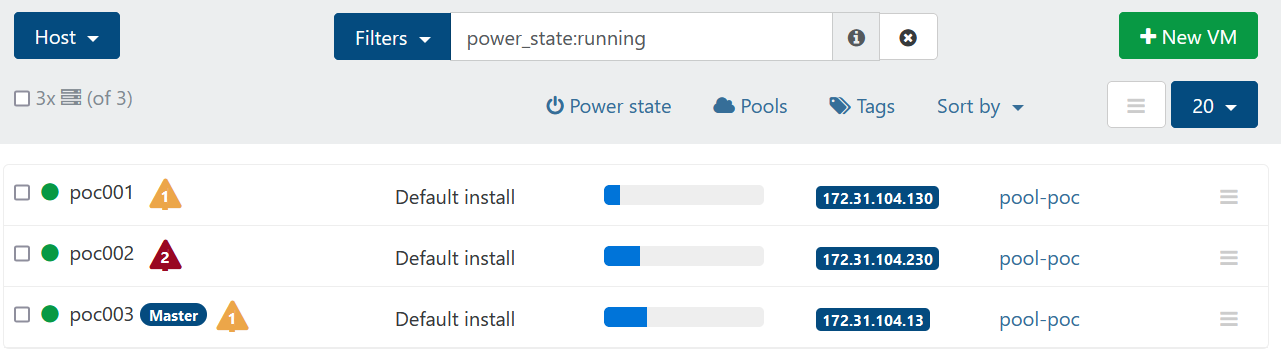
\includegraphics[width=0.9\textwidth]{../poc/nodes-orch.png}
  \caption{Fysieke nodes in Xen Orchestra}
  \label{fig:nodes-list}
\end{figure}

\subsection{Storage in Xen Orchestra}%
\label{sec:storage_orch}
Om iSCSI SAN in te stellen met TrueNAS in Xen Orchestra moet er eerst een iSCSI target worden aangemaakt in de TrueNAS-server. Er wordt hierbij van uitgegaan dat dit al gebeurd is, aangezien dit buiten de scope van deze bachelorproef valt.
Figuur \ref{fig:iscsi-orch} toont de configuratie van het iSCSI target in Xen Orchestra, onder *New Storage*. Hierbij moet het adres en de target van TrueNAS iSCSI worden opgegeven. Dit is het IP-adres van de TrueNAS-server en de naam van het iSCSI target dat eerder is aangemaakt.

\begin{figure}[H]
  \centering
  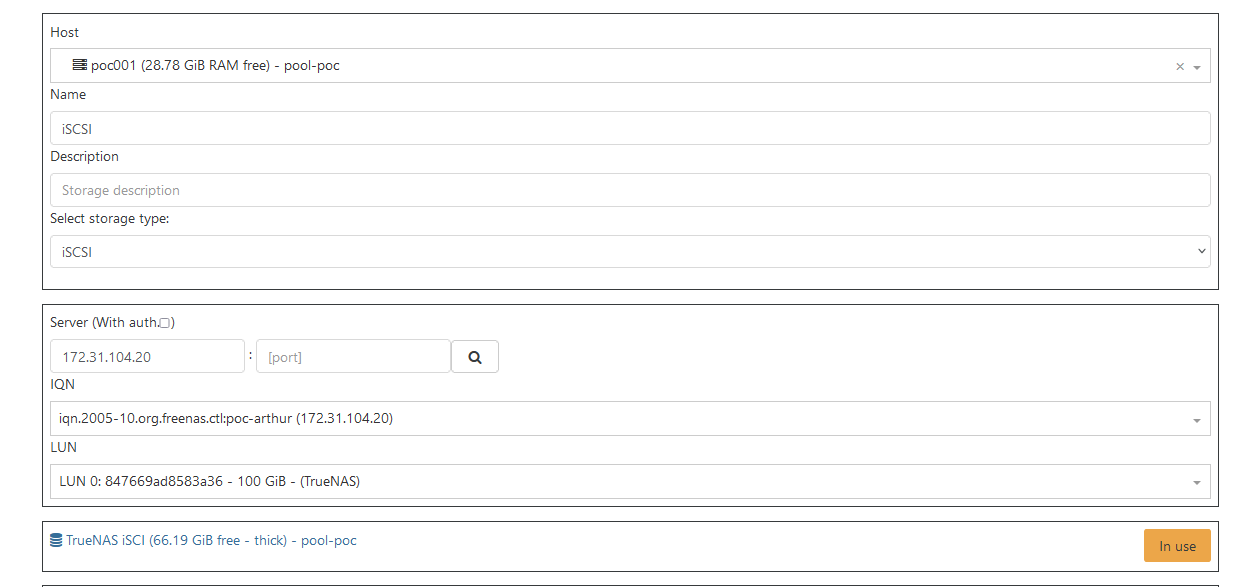
\includegraphics[width=0.9\textwidth, trim=0cm 0cm 20cm 0cm, clip]{../poc/iSCI-orch.png}
  \caption{Storage Area Network met iSCSI in Xen Orchestra}
  \label{fig:iscsi-orch}
\end{figure}  
Hierna wordt de iSCSI-storage toegepast op een virtuele machine. Dit kan gedaan worden door een nieuwe virtuele machine aan te maken of door een bestaande virtuele machine te bewerken.  
In Figuur \ref{fig:vm-storage-orch} is te zien dat de iSCSI storage is toegevoegd aan de virtuele machine. Hierbij wordt de iSCSI storage geselecteerd als schijfopslag.

\begin{figure}[H]
  \centering
  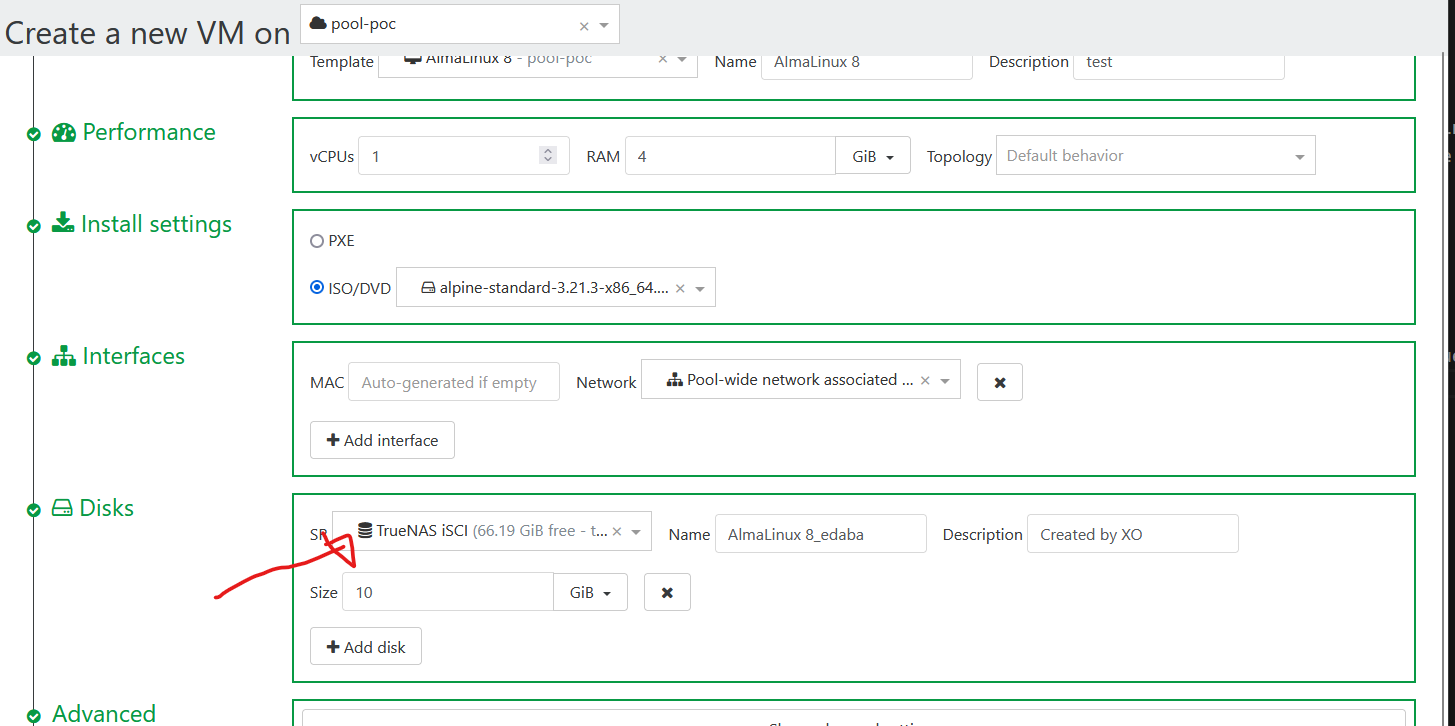
\includegraphics[width=1.0\textwidth, trim=0cm 0cm 15cm 0cm, clip]{../poc/isci-vm-orch.png}
  \caption{Virtuele machineconfiguratie met iSCSI storage in Xen Orchestra}
  \label{fig:vm-storage-orch}
\end{figure}

Hetzelfde principe kan ook worden toegepast voor XOSTOR. Het enige verschil is dat er nu voor elke fysieke node een schijf moet worden toegevoegd. In totaal voor 3 nodes dus 3 extra schijven.  
Eenmaal deze zijn toegevoegd en worden herkend door het operating system, kan er worden overgegaan naar het aanmaken van de XOSTOR storage pool.  
We geven de XOSTOR pool een correcte naam, in de proof of concept is dit *xostor-pool-storage*. Vervolgens moet bij elke node een schijf geselecteerd worden die XOSTOR mag gebruiken.
Let op dat de schijf geen oude partities meer heeft en volledig is geformatteerd; zo niet, zal XOSTOR de schijven niet aanvaarden. Eenmaal toegevoegd, zal Xen Orchestra beginnen met het aanmaken van de XOSTOR storage pool.  
Dit proces kan gemiddeld tot 10 minuten duren. Eenmaal klaar moet het resultaat bekomen worden zoals in Figuur \ref{fig:xostor-pool-orch}.

\begin{figure}[H]
  \centering
  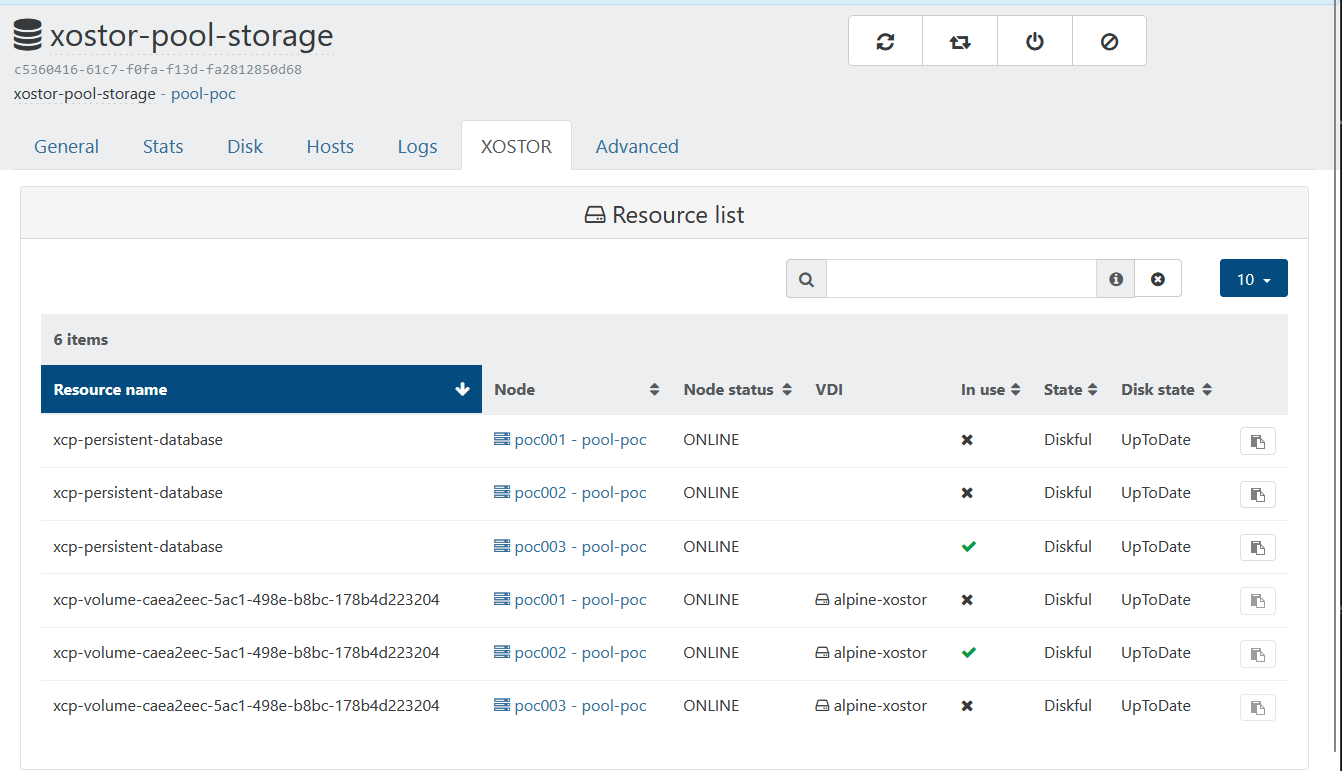
\includegraphics[width=1.0\textwidth, trim=0cm 0cm 13cm 0cm, clip]{../poc/xostor-vieuw-orch.png}
  \caption{XOSTOR pool view in Xen Orchestra}
  \label{fig:xostor-pool-orch}    
\end{figure}

Merk ook op bij Figuur \ref{fig:xostor-pool-orch} dat er al storage is toegewezen aan een virtuele machine op node *poc002*.  
Dit is te bekomen door een virtuele machine aan te maken en de XOSTOR storage pool te selecteren als schijfopslag.  
Dit is op exact dezelfde manier als bij de iSCSI storage pool. Zie Figuur \ref{fig:iscsi-orch}.

Nu zouden er 2 virtuele machines moeten zijn aangemaakt: één met iSCSI storage en één met XOSTOR storage.  
Deze kunnen worden gecontroleerd via de *Home* tab in Xen Orchestra (zie Figuur \ref{fig:virtuelemachines-orch}).

\begin{figure}[H]
  \centering
  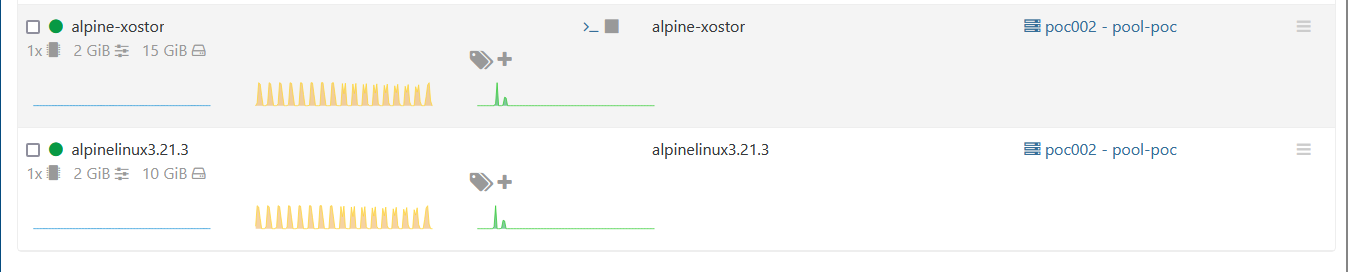
\includegraphics[width=1.0\textwidth, trim=0cm 0cm 17cm 0cm, clip]{../poc/virtuelemachines-orch.png}
  \caption{Lijst van de virtuele machines in Xen Orchestra}
  \label{fig:virtuelemachines-orch}  
\end{figure}

\subsection{High Availability in Xen Orchestra}
\label{sec:ha-orch}
Om een HA-cluster op te zetten in Xen Orchestra moet eerst een pool aangemaakt worden.
Dit kan gedaan worden door naar de tab Pools te gaan en op de knop New Pool te klikken.
Hierin worden de 3 fysieke nodes toegevoegd die eerder zijn aangemaakt. We geven de pool een naam, in dit geval *pool-poc*, zoals te zien is in Figuur \ref{fig:nodes-list}.  
In de pool *Advanced Option* tab wordt de optie *HA* aangezet voor de pool. Nu weet Xen Orchestra dat deze pool een HA-cluster is en dat het de virtuele machines binnen de pool moet beheren volgens het HA-principe.  
*Auto Power-On* en de *Heartbeat* moeten ook aangezet worden. Anders zal Xen Orchestra de virtuele machines niet automatisch opstarten bij een node failure.  
Zie Figuur \ref{fig:ha-settings-orch.png} voor de volledige configuratie van de pool.

\begin{figure}[H]
  \centering
  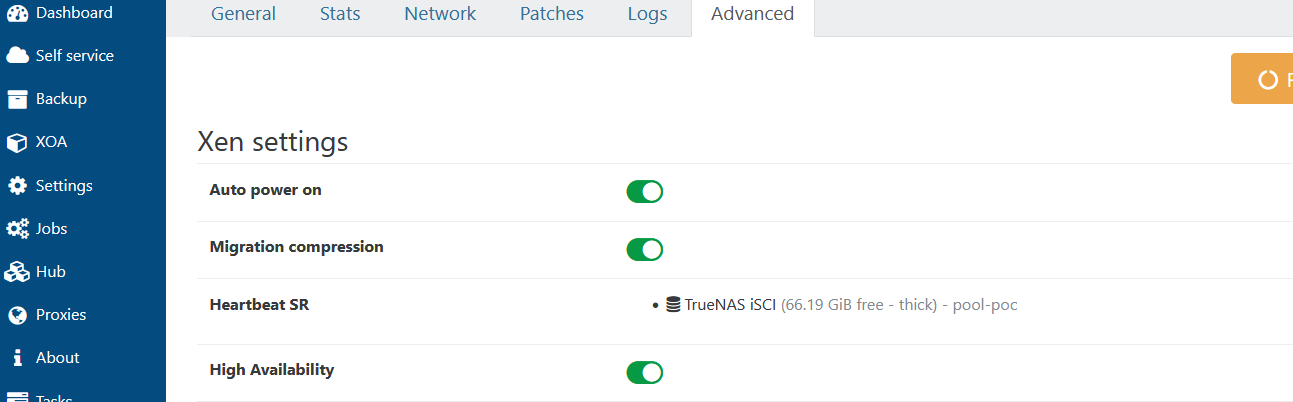
\includegraphics[width=1.1\textwidth, trim=0cm 0cm 10cm 0cm, clip]{../poc/ha-settings-orch.png}
  \caption{High Availability pool in Xen Orchestra}
  \label{fig:ha-settings-orch.png}
\end{figure}
